\documentclass[pdflatex,sn-mathphys,NameDate]{sn-jnl}

\usepackage{graphicx}
\usepackage{multirow}
\usepackage{amsmath,amssymb,amsfonts}
\usepackage{amsthm}
\usepackage{mathrsfs}
\usepackage{xcolor}
\usepackage{textcomp}
\usepackage{manyfoot}
\usepackage{booktabs}
\usepackage{array}
\usepackage{tabularx}
\usepackage{flafter}
\usepackage{placeins}
\raggedbottom
\renewcommand{\topfraction}{.92}
\renewcommand{\bottomfraction}{.65}
\renewcommand{\textfraction}{.07}
\renewcommand{\floatpagefraction}{.78}
\setcounter{topnumber}{2}
\setcounter{totalnumber}{4}
\usepackage{xeCJK}
\setCJKmainfont{Microsoft YaHei}
\graphicspath{{./}}

\begin{document}

\title[ExecKG]{ExecKG: A source-anchored executable grammar resource for GF~0025--2021}

\newcommand{\orc}[1]{\,\href{https://orcid.org/#1}{\textrm{\mdseries\scriptsize #1}}}
\author[1]{\fnm{Tingrui} \sur{You}\orc{0009-0006-0521-2194}}
\author[2]{\fnm{Na} \sur{Zhang}\orc{0009-0007-1598-2907}}
\author[2]{\fnm{Ling} \sur{Xiong}\orc{0000-0001-9900-2978}}
\author*[2]{\fnm{Jimei} \sur{Li}\orc{0000-0003-1222-635X}}\email{ljm@blcu.edu.cn}

\affil[1]{\orgname{Hainan International College, Beijing Language and Culture University}, \orgaddress{\country{China}}}
\affil*[2]{\orgname{School of Information Science, Beijing Language and Culture University}, \orgaddress{\city{Beijing}, \country{China}}}

\abstract{Teaching-grammar standards provide an authoritative inventory, but their prose is not directly executable or source-auditable. We present ExecKG, a source-anchored executable grammar resource for GF~0025--2021. It represents 572 official grammar points as 646 diagnostic units with profiles, runtime bindings, source/page anchors, and 4,522 contract checks generated by 233 templates. The resource separates inventory-wide compilation from candidate-level validation. On a frozen benchmark of 3,000 supplied candidates covering 37 labels, three annotators reach 70.43\% exact agreement and Gwet's AC1 of 0.779. A character SVM augmented with executor features reaches 91.08 macro-F1, a pooled gain of 2.09 points over a text-only SVM (95\% grouped interval $[0.84,3.40]$); its 0.98-point difference from MacBERT is uncertain. On 244 author-written candidates, the frozen executor reaches 59.89 macro-F1, whereas the handbook-trained SVM reaches 39.03, revealing limited transfer beyond the benchmark conditions. The release provides compiler inputs, binding summaries, contract tests, source metadata, hashes, predictions, and verification scripts; licensed standard and sentence text remain outside the package. ExecKG is intended as auditable infrastructure for Chinese grammar-point verification, with behavioral conclusions bounded to the released benchmark.}

\keywords{language resources, Chinese grammar, knowledge graphs, executable constraints, annotation agreement, grammar-point verification}

\maketitle

\section{Introduction}
\label{sec:intro}

\begin{figure}[!ht]
\centering
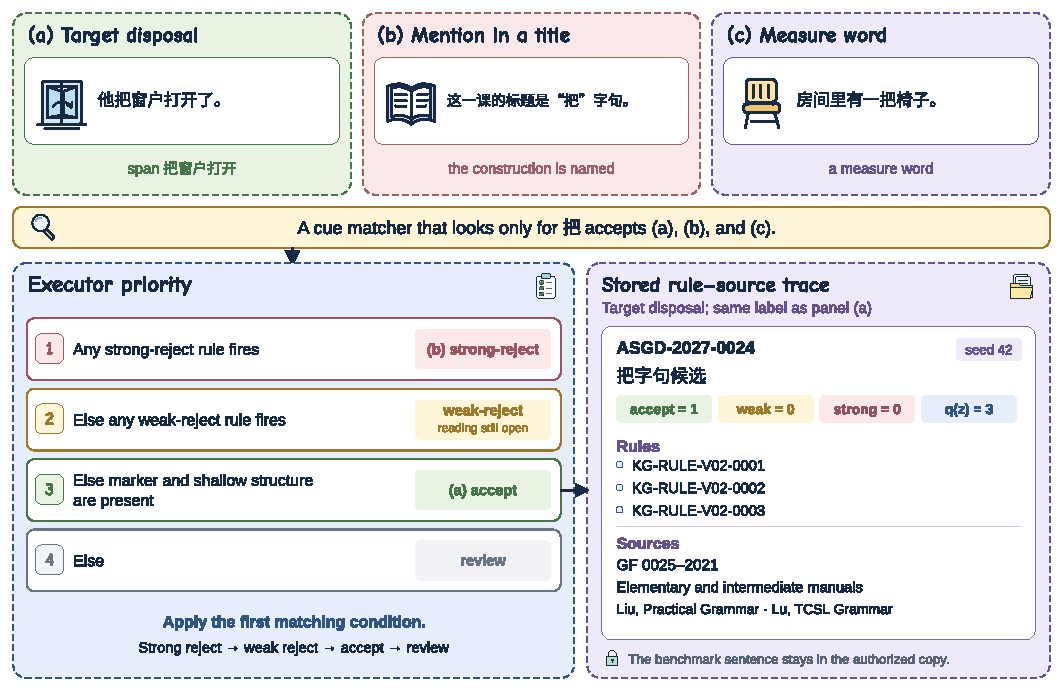
\includegraphics[width=\columnwidth]{fig_concept.pdf}
\caption{Three readings of \mbox{把}, the executor priority, and the stored trace for a target disposal. Sentences (a)--(c) illustrate the readings. The trace is benchmark item ASGD-2027-0024, which carries the same label as (a). Section~\ref{sec:walkthrough} reports the executor and SVM outputs on (a)--(c).}
\label{fig:concept}
\end{figure}

GF~0025--2021 organizes 572 grammar points by category and proficiency level, and the accompanying handbooks add construction formats, examples, and usage notes~\citep{moe2021gf,cti2022handbooks,wang2023syllabus,jin2021principles}.
A teacher or a program still has to decide whether a particular span realizes one of those points.
ExecKG makes that decision for a candidate that is already in hand: a sentence, a span, a proposed grammar point, and a diagnostic family.
The executor records the state, the rule identifiers, and the source anchors that fired.
The benchmark score comes from a linear SVM that reads character features together with those executor fields.
Figure~\ref{fig:concept} is the case the rest of the paper follows.

Chinese grammatical error diagnosis locates learner errors~\citep{yu2014overview,rao2017ijcnlp,liang2020bert}.
A prompted model can add a correction and a rationale.
Those outputs answer a different question from whether the span in (a) is the disposal point, and they are not designed or evaluated for the candidate-verification task in this paper.
Section~\ref{sec:walkthrough} shows the record ExecKG stores for a target disposal of the kind in (a).
Sections~\ref{sec:benchmark} and~\ref{sec:eval} test that decision on 3,000 supplied candidates and on 244 author-written candidates.

The compiler covers all 572 official points with 646 diagnostic units, 233 templates, and 4,522 passing contract tests.
The graph contains 35,379 nodes and 72,898 edges and keeps an earlier release as a subgraph.
On the benchmark, an SVM that reads the executor state reaches 91.08 macro-F1, 2.09 points above a text-only SVM.
The same mean is 0.98 points above MacBERT, and that interval includes zero.
On the 244 author-written candidates, the frozen executor reaches 59.89 macro-F1, and 65.92 on the 148 candidates that use the 37 benchmark labels.

The paper makes three resource contributions.
First, it specifies a versioned compilation interface that connects an official point to a diagnostic profile, a runtime binding, a contract-test record, and a source anchor.
Second, it releases a copyright-aware package containing the compiler inputs, summaries, test records, predictions, hashes, and verification scripts needed to audit and reuse that interface.
Third, it separates inventory-wide compilation from behavioral validation and reports both benchmark performance and transfer to 244 author-written candidates.
The central claim is therefore about an auditable resource interface and its bounded utility for candidate-conditioned verification; the 3,000-candidate benchmark does not constitute behavioral validation of all 572 points.

\section{Related resources}
\label{sec:related}

Figure~\ref{fig:concept} needs four things that existing resources split apart: a named point, a span, a decision, and a source for the decision.
Table~\ref{tab:compare} places ExecKG against the resources it builds on.

\begin{table}[!ht]
\centering
\small
\hyphenpenalty=10000\exhyphenpenalty=10000
\begin{tabularx}{\textwidth}{@{}>{\raggedright\arraybackslash}p{0.16\textwidth}>{\raggedright\arraybackslash}X>{\raggedright\arraybackslash}X>{\raggedright\arraybackslash}X@{}}
\toprule
Resource & Constraint & Interface & What is checked \\
\midrule
GF~0025--2021 & Official inventory in prose & Read by a person & The published standard \\
Handbooks & Formats, examples, and notes & Read by a person & Editorial examples \\
CGED & Error type and location & Shared-task systems & Learner sentences \\
ExecKG & Binding per diagnostic unit & Executor on a supplied candidate & 3,000 benchmark candidates and 244 author-written candidates \\
\bottomrule
\end{tabularx}
\caption{Comparison on identifier, constraint form, interface, and the text each resource is checked against. ExecKG public fields are the identifiers, bindings, traces, predictions, and the 244 author-written candidates in the supplementary package.}
\label{tab:compare}
\end{table}

CGED shared tasks established detection and location for four broad learner-error types~\citep{yu2014overview,rao2017ijcnlp}.
Later models added pretrained encoders, dependency graphs, and prompted correction~\citep{liang2020bert,luo2020graph,mu2024llm}.
Those systems take a learner sentence and return an error type and a location.
Table~\ref{tab:compare} lists those types and locations as the content the shared tasks supply.
In Figure~\ref{fig:concept} the proposed grammar point is already attached to the span, and the question is whether that span realizes the point.

The standard and the handbooks state what should be taught~\citep{moe2021gf,cti2022handbooks,wang2023syllabus,jin2021principles}.
Table~\ref{tab:compare} compares those sources, and CGED, on constraint form, interface, and the text each one is checked against.
The graph lineage is internal.
Version~2, an inventory graph of 28,158 nodes and 64,046 edges, is retained as a subgraph and is not part of the public node table.
Version~3 adds the compilation layer: 7,221 nodes and 8,852 edges, namely 646 diagnostic units, 646 profiles, 233 templates, 646 runtime bindings, 4,522 contract tests, 524 unique handbook-page anchor records supporting 572 point alignments, and 4 catalog corrections.
The compiled graph is that sum, 35,379 nodes and 72,898 edges.
The public release does not include the full node table or the full edge table.
Knowledge graphs and neuro-symbolic predictors attach rules to learned decisions~\citep{hogan2021kg,hu2016rules}.
Compilation is the step that turns a page of the standard into a constraint the executor can fire, and that keeps the page with the firing.
Explanation research separates a plausible rationale from evidence tied to the decision~\citep{fei2023explanations,jacovi2020faithfulness,lyu2024faithful}.
ExecKG stores the fired rule identifiers and source anchors with the graph version.
\citet{olausson2023linc} and \citet{zhang2025qcompiler} compile natural language into logic or a query tree for a different task.
ExecKG compiles a teaching-grammar standard into the candidate decision above.

\section{The ExecKG resource}
\label{sec:resource}

\subsection{Task}
\label{sec:task}

Take sentence (a) in Figure~\ref{fig:concept}.
The instance is $z=(x,c,g,f)$: the sentence $x$, the span $c=\mbox{把窗户打开}$, the proposed point $g$, and the disposal family $f$.
Each family belongs to one regime.
Disposal is structural-pattern: the decision includes the target label and the quality of the span boundary.
Temporal and locative families are complex-functional: the decision asks whether the expression fills the target role.
Both regimes return a binary target status.
The full output is
\begin{equation}
\hat{Y}=\{\hat{y}_{t},\hat{y}_{e},\hat{y}_{f},\hat{y}_{v},\hat{y}_{s},\hat{b}_{s},\tau\},
\label{eq:output}
\end{equation}
where $\hat{y}_{t}$ is target status, $\hat{y}_{e}$ extraction, $\hat{y}_{f}$ function, $\hat{y}_{v}$ evidence support, $\hat{y}_{s}$ slot status, $\hat{b}_{s}$ the slot span, and $\tau$ the rule--source trace.
The primary metric scores $\hat{y}_{t}$.
Extraction, function, evidence support, and slot status are companion outputs.
The experiments score candidates that are already marked.
Finding the span in an unmarked document is a separate task.

\subsection{Authority inventory}

\begin{figure}[!ht]
\centering
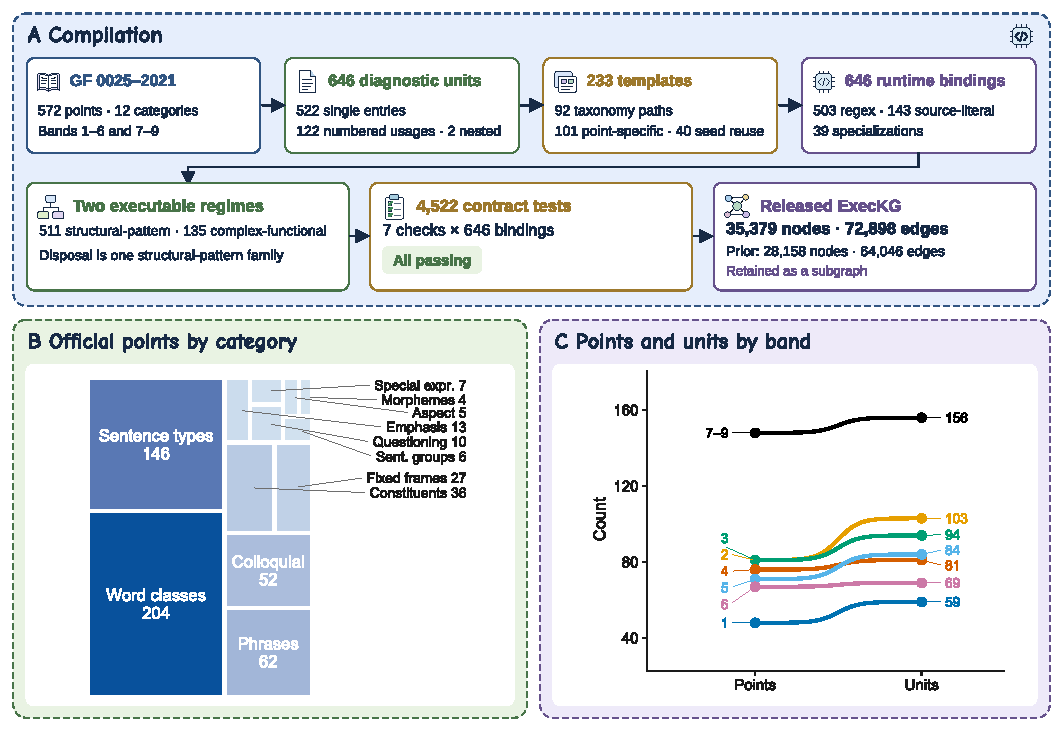
\includegraphics[width=\columnwidth]{fig_pipeline.pdf}
\caption{Compilation of GF~0025--2021. Panel A is the path from the official inventory to the released graph. Panel B is the category composition of the 572 points. Panel C compares points with diagnostic units inside each proficiency band.}
\label{fig:pipeline}
\end{figure}

The authority layer stores the official identifier, taxonomy path, and provenance for all 572 points, 12 categories, 33 subitems, and 103 taxonomy paths.
Figure~\ref{fig:pipeline} follows that inventory from the official points to the graph.
Levels~1 through~6 follow the numbered bands of the standard, and levels~7--9 are stored as one band.
Word classes and sentence types account for 350 of the 572 points.
The six smallest categories are emphasis (13), questioning (10), special expressions (7), sentence groups (6), aspect (5), and morphemes (4).
Table~\ref{tab:bands} gives the point and unit counts at both ends of each band in Figure~\ref{fig:pipeline}.
The benchmark in Section~\ref{sec:benchmark} scores eight diagnostic families and 37 experimental labels.
Disposal, the family of Figure~\ref{fig:concept}, is one of those families.

\begin{table}[!ht]
\centering
\small
\begin{tabular}{lrr}
\toprule
Band & Points & Units \\
\midrule
1 & 48 & 59 \\
2 & 81 & 103 \\
3 & 81 & 94 \\
4 & 76 & 81 \\
5 & 71 & 84 \\
6 & 67 & 69 \\
7--9 & 148 & 156 \\
\midrule
Total & 572 & 646 \\
\bottomrule
\end{tabular}
\caption{Official points and diagnostic units by proficiency band. Levels 7--9 are stored as one band.}
\label{tab:bands}
\end{table}

\subsection{Profiles, bindings, and templates}

A profile stores the regime, triggers, typed slots, acceptance conditions, weak-reject conditions, strong-reject conditions, and confusable uses.
A runtime binding is the detector that executes for that profile.
Figure~\ref{fig:pipeline} counts the bindings, the two regimes, and the three template origins.
The experiments use a coarser cut of the regime field: seven structural families, and temporal and locative expressions as the complex-functional family.
Disposal, the family in Figure~\ref{fig:concept}, is one of the seven.
The 233 templates are produced by a deterministic compiler.
Its inputs are the official catalog, a constraint file, and a correction table.
The constraint file stores the rule content for the 37 seed labels and the taxonomy templates.
The program instantiates each template from those inputs and records its origin, regime, slot schema, and positive, weak, and strong conditions, with status \texttt{machine\_instantiated\_source\_anchored}.
The compiler can be rerun on those three inputs.
The generated binding is the executable layer for the inventory.
A compilation path in the graph runs from the official point to a diagnostic unit, a profile, a runtime binding, and an authority source.
Contract tests hang off the binding, and handbook-page anchors hang off the official point.

Each binding receives seven synthetic checks: schema, detector invocation, positive matching, negative gating, and the diagnosis branches.
All 4,522 tests pass.
They confirm that the binding behaves as specified when the evidence state is given.
The profile schema names seven diagnosis labels.
The experiment executor returns four states and writes four of those labels, as Table~\ref{tab:diagnosis} records.
The other three labels are the contract-test branches under a supplied evidence state.

\begin{table}[!ht]
\centering
\small
\begin{tabular}{ll}
\toprule
Profile diagnosis & Where the experiment uses it \\
\midrule
目标用例 & accept \\
边界问题 & weak-reject \\
表层触发但非目标 & strong-reject \\
不确定/需复核 & review \\
结构缺槽 & contract test, supplied evidence state \\
语义不兼容 & contract test, supplied evidence state \\
其他具体构式 & contract test, supplied evidence state \\
\bottomrule
\end{tabular}
\caption{Seven profile diagnoses and the four executor states. The experiment executor writes the first four labels. The last three are checked when the contract test supplies the evidence state.}
\label{tab:diagnosis}
\end{table}

\subsection{Anchors, repairs, and lineage}

Every official point has a handbook alignment: 569 links are high confidence and three are medium confidence.
The source anchors are 362 OCR point pages and 210 confirmed appendix spans.
The public alignment keeps the page identifier, the score, and a page hash.
Two catalog fields were corrected against the appendix.
For GF0025-2021-5-010, 【五10】将, the section is 引出施事、受事 on appendix page 223.
For GF0025-2021-3-002, 【三02】, the suffix list is 儿、家、们、头、子 on appendix page 198.

The present graph has 35,379 nodes and 72,898 edges.
It contains the previous internal inventory graph, 28,158 nodes and 64,046 edges, as a subgraph.
The public summary reports the totals and the subgraph relation.
Sentence nodes in that subgraph carry licensed text, so the node table stays with the authorized copy.
Section~\ref{sec:related} lists the node types added in the compilation layer.

The crosswalk sets \texttt{review\_status} to \texttt{not\_claimed} on all 646 units.
Inside the 37-label benchmark, 16 point-specific bindings were reviewed.
Positive sentence--point pairs in the authorized annotation cover 219 official points, 3,645 unique pairs.
The other 353 points have no released positive sentence.
The public summary keeps the counts, a sample of unsalted SHA-256 hashes, and the workbook hash.
Table~\ref{tab:coverage} keeps these layers separate.
The 37 experimental labels are not 37 of the 572 official points, and Section~\ref{sec:eval} scores that benchmark.

\begin{table}[!ht]
\centering
\small
\hyphenpenalty=10000\exhyphenpenalty=10000
\begin{tabularx}{\textwidth}{@{}>{\raggedright\arraybackslash}p{0.28\textwidth}>{\raggedright\arraybackslash}p{0.22\textwidth}>{\raggedright\arraybackslash}X@{}}
\toprule
Layer & Scope & What is checked \\
\midrule
Official inventory & 572 points & Identifier, level, and taxonomy path \\
Compiled units & 646 units, 233 templates & Profile, binding, and source anchor \\
Contract tests & 4,522 & Binding behavior when the evidence state is given \\
Positive pairs & 219 points, 3,645 pairs & A released positive sentence--point pair exists \\
No released positive sentence & 353 points & Count in the public summary \\
Reviewed bindings & 16 point-specific bindings & Review recorded inside the benchmark \\
Specification review & 646 units & Two raters compare each profile with its cited page; Table~\ref{tab:specreview} \\
Behavioral evaluation & 37 labels, 3,000 candidates & Target-status macro-F1 \\
Crosswalk status & 646 units & \texttt{review\_status} is \texttt{not\_claimed} \\
\bottomrule
\end{tabularx}
\caption{Coverage and validation layers. A count in one row does not stand in for a count in another.}
\label{tab:coverage}
\end{table}

Two raters compared every profile with the page named in its anchor.
They agreed on 387 of the 646 units.
A third rater decided the other 259.
Table~\ref{tab:specreview} is that record.
The crosswalk field \texttt{review\_status} remains \texttt{not\_claimed}, so the release check is unchanged.
Of the 215 coarse anchors, 151 are taxonomy instantiations, 46 are point-specific, and 18 reuse a seed label.
Each of those 215 anchors is the range GF~0025--2021 PDF pp.~176--259.
Eight units mismatch the cited entry.
Seven of them reuse a seed label.
Each of the eight now has a unit-level rewrite checked against its entry.
That rewrite is kept apart from the compiler inputs hashed on 26 September 2026, and Section~\ref{sec:eval} scores that frozen release.
Four of them cite a point page: 【二24】 on p.~188, 【三49】 on p.~206, and both patterns of 【六40】 on p.~239.
【五40】, 【五41】, 【七—九35】, and the 为……所 pattern of 【七—九36】 still cite the appendix range pp.~176--259.
None of the 3,000 benchmark candidates proposes these eight official points, so the released test predictions are unchanged.
The other 55 units keep the cited condition and need a wording repair, 40 of them taxonomy instantiations and 15 seed-reuse units.

\begin{table}[!ht]
\centering
\small
\begin{tabular}{lr}
\toprule
Final judgment & Units \\
\midrule
Consistent with the cited page & 368 \\
Wording repair, condition unchanged & 55 \\
Condition mismatches the entry & 8 \\
Page anchor too coarse to check & 215 \\
\midrule
Total & 646 \\
\bottomrule
\end{tabular}
\caption{Specification review of the 646 diagnostic units. The first two raters agreed on 387 units. The remaining 259 were adjudicated.}
\label{tab:specreview}
\end{table}

This audit records consistency with the cited source and the disposition of an anchor; it is not a claim that every generated profile has been linguistically adjudicated.

\subsection{Executor}
\label{sec:executor}

For a candidate $z$, let $P(z)$, $W(z)$, and $S(z)$ be the fired positive, weak-reject, and strong-reject rule sets.
The evidence score is
\begin{equation}
q(z)=|P(z)|-|W(z)|-2|S(z)|.
\label{eq:score}
\end{equation}
The executor applies Table~\ref{tab:states} in order.
The score $q(z)$ is kept as a feature of the candidate.
If an accept flag and a weak-reject flag are both true, the reported state is weak-reject.

\begin{table}[!ht]
\centering
\small
\begin{tabular}{@{}p{0.58\columnwidth}l@{}}
\toprule
Condition, in order & State \\
\midrule
Any strong-reject rule fires & strong-reject \\
Otherwise any weak-reject rule fires & weak-reject \\
Otherwise the marker and the shallow structure are present & accept \\
Otherwise & review \\
\bottomrule
\end{tabular}
\caption{Executor state map. The four states follow this order over fired rules. Equation~\ref{eq:score} is recorded alongside the state. When the proposed label has a binding, the structure flag is that binding's structure pattern. For \mbox{把字句候选} the pattern is \mbox{把} followed by at least two characters. A label without a binding uses the fallback: the shortest marker is present and the candidate is at least one character longer than that marker.}
\label{tab:states}
\end{table}

\subsection{Walkthrough}
\label{sec:walkthrough}

Apply Table~\ref{tab:states} to Figure~\ref{fig:concept}.
Sentences (a)--(c) illustrate three readings of \mbox{把}.
They are not benchmark items.
The \mbox{把字句候选} binding sets the structure flag when \mbox{把} is followed by at least two characters.
The frozen executor accepts all three sentences: the marker and the structure pattern are both present, and no strong-reject rule fires.
SVM+ExecKG, refit at the released value of $C$ for each seed, labels (a) as target on seeds 13, 42, and 2027.
It labels (c) as target on those three seeds.
It labels (b) as non-target on seeds 13 and 42, and as target on seed 2027.
The stored trace below is not a run on (a)--(c).

The disposal test item ASGD-2027-0024, from seed 42, is a benchmark candidate with the same label as (a), \mbox{把字句候选}.
Its sentence stays in the authorized copy.
The gold label and the SVM prediction are both target.
The flags are accept $=1$, weak-reject $=0$, and strong-reject $=0$, so the executor state is accept and $q(z)=3$.
The stored trace is:
\begin{quote}\raggedright\footnotesize
candidate:把字句候选; family:处置/受事重组构式;
rule:KG-RULE-V02-0001; rule:KG-RULE-V02-0002; rule:KG-RULE-V02-0003;
source:REF-GF0025-2021; source:REF-GRAMMAR-MANUAL-ELEM;
source:REF-GRAMMAR-MANUAL-INTER; source:REF-LIU-PRACTICAL-GRAMMAR;
source:REF-LU-TCSL-GRAMMAR.
\end{quote}
Rules 0001--0003 are the positive set for that item.
The executor writes a record of this form for the candidate it evaluates: the candidate label, the family, the fired rule identifiers, and the source identifiers.
REF-GF0025-2021 is the standard~\citep{moe2021gf}.
REF-GRAMMAR-MANUAL-ELEM and REF-GRAMMAR-MANUAL-INTER are the elementary and intermediate volumes of the Grammar Learning Handbooks~\citep{cti2022handbooks}.
REF-LIU-PRACTICAL-GRAMMAR is \citet{liuPractical}, and REF-LU-TCSL-GRAMMAR is \citet{luTcsl}.
The trace is the executor evidence supplied to the classifier in Equation~\ref{eq:clf}.
On this item the SVM prediction matches the gold label.
The trace records which rules fired.
It is not a decomposition of the SVM weight vector.

\subsection{Public fields and license}

Author-created tables and JSON are released under CC~BY~4.0.
Code is released under the BSD 3-Clause License.
Table~\ref{tab:release} is the boundary a reuser can rely on.
Table~\ref{tab:reuse} separates three uses of that package.
The trace in Section~\ref{sec:walkthrough} shows the rule identifiers and the source anchors that travel with an evaluated candidate.
The check is \texttt{python scripts/verify\_release.py} on CPython~3.12.13.

\begin{table}[!ht]
\centering
\small
\hyphenpenalty=10000\exhyphenpenalty=10000
\begin{tabularx}{\textwidth}{@{}>{\raggedright\arraybackslash}p{0.30\textwidth}>{\raggedright\arraybackslash}X@{}}
\toprule
Use & What the release provides \\
\midrule
Audit & Identifiers, template records, page hashes, sentence-group hashes, consolidated labels, rule traces, predictions, and agreement tables \\
New marked candidate & Compiler, constraint file, correction table, and executor. The user supplies the sentence, the span, the proposed point, and the family \\
Reported scores & Predictions paired with the consolidated labels, so the published metrics can be recomputed \\
\bottomrule
\end{tabularx}
\caption{Three uses of the release. Benchmark sentences remain in the authorized copy, as Table~\ref{tab:release} states, so a new sentence is one the user supplies.}
\label{tab:reuse}
\end{table}

\begin{table}[!ht]
\centering
\small
\hyphenpenalty=10000\exhyphenpenalty=10000
\begin{tabularx}{\textwidth}{@{}>{\raggedright\arraybackslash}X>{\raggedright\arraybackslash}X@{}}
\toprule
Released & Withheld \\
\midrule
Official identifiers, taxonomy paths, and template records & Standard page images and handbook prose \\
Page anchors, alignment scores, and page hashes & Benchmark sentences and candidate spans \\
Normalized sentence hashes and consolidated labels & Annotator free text and copied slot strings \\
Rule traces, predictions, and agreement tables & Raw API prompts and responses \\
244 author-written candidates and the 646-unit review record & Benchmark sentences and candidate spans \\
Graph totals and the subgraph relation & Full node and edge tables \\
\bottomrule
\end{tabularx}
\caption{Release boundary. Counts and identifiers support audit. Licensed wording and sentence text remain in the authorized copies.}
\label{tab:release}
\end{table}

\section{Benchmark}
\label{sec:benchmark}

\subsection{Construction}

The benchmark contains 3,000 candidates, 37 experimental labels, and eight families.
Temporal and locative expressions form the complex-functional regime in the experiments.
The other seven families form the structural-pattern regime.
The eight families are the evaluation cut.
The twelve categories in Figure~\ref{fig:pipeline} are the official taxonomy.
Each benchmark name ends in 候选.
The name for the disposal in Figure~\ref{fig:concept} is \mbox{把字句候选}.
Official identifiers keep the form GF0025-2021.
Appendix~\ref{app:labels} lists the full set.

Seven families were taken from the three Grammar Learning Handbooks with fixed regular expressions~\citep{cti2022handbooks}.
Duplicate sentence--family--span rows were removed.
Inside each family quota, ranking preferred short, sentence-like lines and pages whose topic cue matched the family.
The ranking did not look at the label.
Ties used seed 20260629.
The 650 temporal and locative candidates came from an earlier pool, recorded separately from those handbook quotas.
The quotas are a diagnostic sample of the constructions, including disposal.
The seven handbook families and the rules drawn from the same handbooks therefore share that documentation.
The grouped split, defined below, keeps one normalized sentence in one split.
It leaves candidates from the same page, and sentences that still differ after normalization, free to fall in different splits.

The 3,000 candidates fall in 2,557 normalized sentence groups.
The consolidated target distribution is 2,539 target, 457 non-target, and four review cases.
Review cases are excluded from supervised target scoring.
Evidence-support decisions were collected on a stratified subset of 1,000 candidates.
Slot annotation produced 1,320 slot rows on those candidates.

A separate set contains 244 author-written candidates.
The sentences are outside the three handbooks and outside the 3,000 benchmark items.
They cover the 37 experimental labels and 24 further official points, two from each of the 12 categories.
Compiler inputs were hashed on 26 September 2026, before these labels were read.
Two raters agreed on 228 of the 244 items.
Adjudication of the other 16 leaves 122 target and 122 non-target labels.
The gold matches that construction plan on all 244 items.
Table~\ref{tab:external} scores the frozen executor and the refit SVMs on this set, apart from the 3,000-candidate benchmark.

\subsection{Annotation and agreement}

\begin{figure}[!ht]
\centering
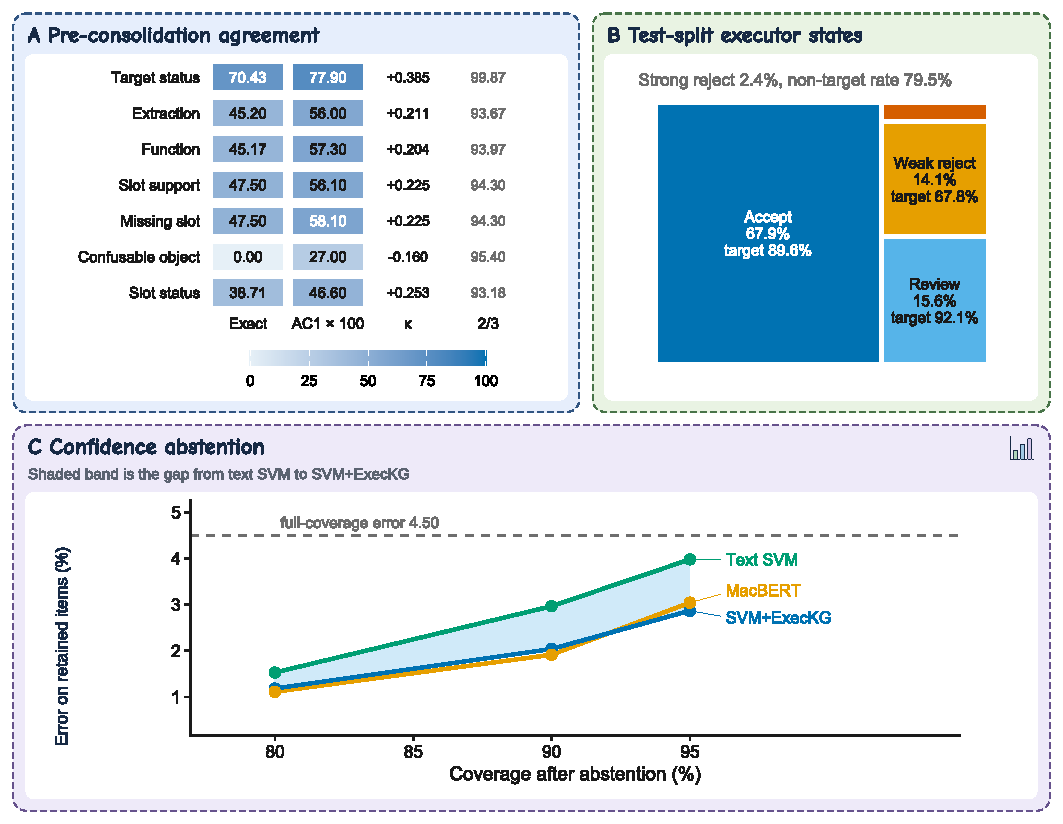
\includegraphics[width=\columnwidth]{fig_operation.pdf}
\caption{Agreement, executor states, and confidence abstention. Panel A shows exact three-annotator agreement and AC1 on a 0--100 scale; kappa and the two-of-three adjudication rate are printed beside the tiles. Panel B is the state mix on the test splits. Panel C abstains by classifier confidence. The shaded band is the gap from text SVM to SVM+ExecKG, and the dashed line is the full-coverage error of SVM+ExecKG.}
\label{fig:operation}
\end{figure}

Three annotators passed a qualification screen and two calibration rounds.
Consolidation kept unanimous labels, otherwise the majority, otherwise a predesignated resolver.
On target status, the field that decides Figure~\ref{fig:concept}, at least two of the three annotators give the same label on 99.87\% of items.
That figure is the share of items the majority rule can resolve.
Exact agreement of all three annotators is 70.43\%.
Fleiss' $\kappa$ is 0.385 and Gwet's AC1 is 0.779~\citep{fleiss1971kappa,gwet2008ac1}.
AC1 is the primary coefficient because the label distribution is unbalanced: a global majority classifier already reaches 85.21\% accuracy, and $\kappa$ falls when one class dominates.
Figure~\ref{fig:operation} gives every annotated field.
Target status is the consolidated label for the primary metric.
Extraction, function, evidence support, slot status, and confusable object are companion fields.
Confusable object has exact agreement 0.00\%, $\kappa=-0.160$, and AC1 0.270.
Those companion fields are released with the agreement in Figure~\ref{fig:operation}.
They are not a second gold standard for the primary metric.
The companion scores in Section~\ref{sec:eval} compare models with these consolidated labels.
Confusable object has exact agreement of zero and is an exploratory field.

\subsection{Splits, features, and metrics}

Repeated sentences would make a random row split optimistic.
Each sentence is normalized and hashed, and the hash is the group.
Normalization applies Unicode NFKC, lowercases the string, maps common full-width punctuation to ASCII, and deletes whitespace.
The group identifier is the first 16 hexadecimal characters of the SHA-1 digest of that string.
For seeds $\{13,42,2027\}$, grouped splits yield 2,097 training candidates, 299--300 development candidates, and 599--600 test candidates, with no shared group.

The primary metric is target-status macro-F1.
Hard-negative accuracy is recall of the non-target class.
Development macro-F1 selects $C\in\{0.25,1,4\}$ for logistic regression and SVM.
The text representation concatenates the sentence, the span, the proposed point, and the family.
A character TF--IDF encoder uses 1--4 grams, minimum document frequency 2, sublinear term frequency, and at most 100,000 features.
The marker bundle keeps point and family identity, candidate geometry, marker and structure checks, and binding coverage together.
The executable bundle adds the four-state flags, $q(z)$, the diagnosis label, and the fired rule identifiers, the same fields stored for ASGD-2027-0024.
A class-balanced linear classifier predicts
\begin{equation}
\hat{y}=\arg\max_{y} w_{y}^{\top}[\phi_{\mathrm{char}}(z);\phi_{\mathrm{KG}}(z)].
\label{eq:clf}
\end{equation}
The primary model is a linear SVM~\citep{cortes1995svm}.
Logistic regression is used for the staged ablation so that every stage shares one classifier.
MacBERT is fine-tuned for five epochs with batch size 16, learning rate $2\times10^{-5}$, weight decay 0.01, 10\% warmup, and maximum length 128~\citep{cui2020macbert}.
The best development checkpoint is kept.

Uncertainty uses 5,000 bootstrap resamples of sentence groups~\citep{koehn2004significance}.
Per-seed intervals below resample groups inside that seed's test split, with analysis seed 20270718.
The pooled interval estimates the mean of the three split-level differences.
Each pooled draw samples the union of 1,259 test groups once, with replacement, and gives a group the same weight in every seed where that group appears.
The interval is the 2.5 and 97.5 percentiles of the mean of the three differences, from 5,000 draws with analysis seed 20270926.
The test groups overlap: seeds 13 and 42 share 85 groups, seeds 13 and 2027 share 107, seeds 42 and 2027 share 95, and 15 groups appear in all three tests.
Each test contains 510 or 511 groups.
Panel B of Figure~\ref{fig:operation} shows the executor-state mix on the test splits.
Across the full 3,000 candidates, 2,251 (75.0\%) fire at least one runtime rule.

\section{Evaluation}
\label{sec:eval}

\subsection{Main comparison}

\begin{figure}[!ht]
\centering
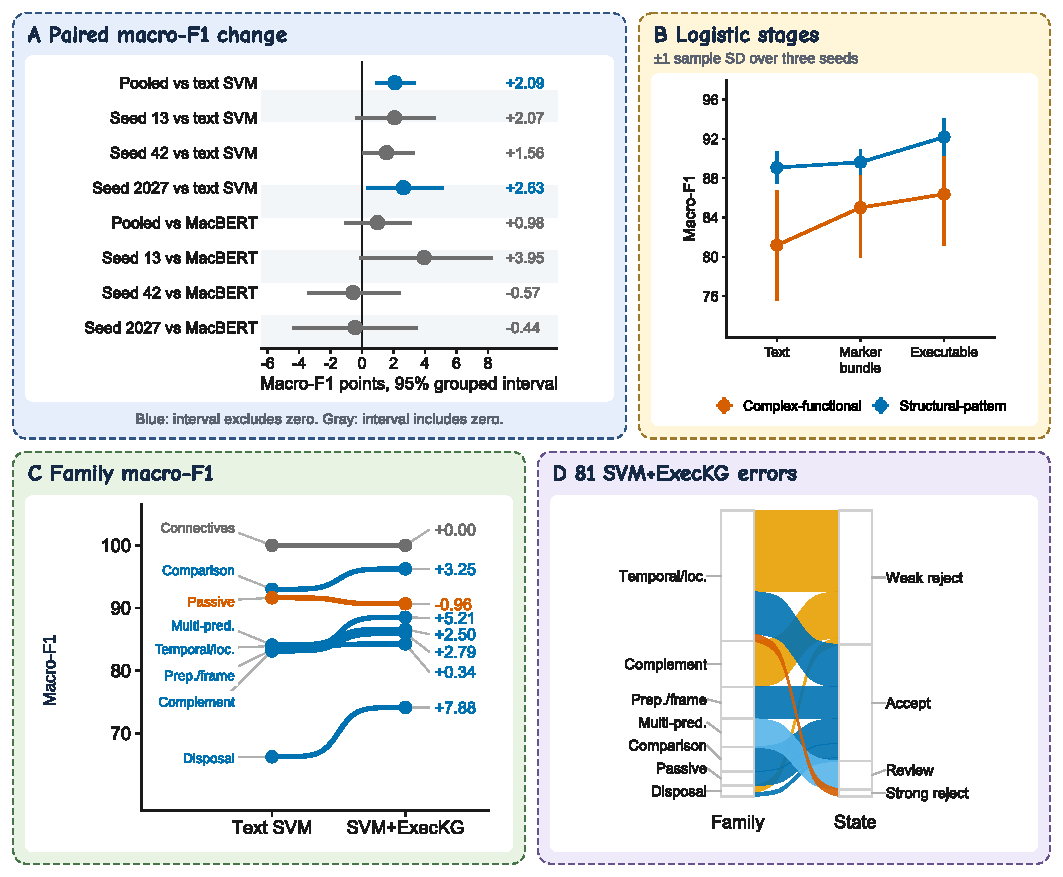
\includegraphics[width=\columnwidth]{fig_results.pdf}
\caption{Target-status results. In panel A, blue intervals exclude zero and gray intervals include zero. The pooled bars use the earlier independent resamples; their signs match the shared-weight intervals in the text. Intervals in panel B are three-seed sample standard deviations. Family slopes in panel C have no per-family paired interval. Panel D pools 81 errors from the three test splits; connectives contribute none.}
\label{fig:results}
\end{figure}

Figure~\ref{fig:results} and Table~\ref{tab:ladder} place SVM+ExecKG against majority classes, the executor alone, text-only linear models, and MacBERT.
SVM+ExecKG obtains 91.08 macro-F1 (sample standard deviation 0.83) and 85.52 hard-negative accuracy.
The pooled gain over text-only SVM is $+2.09$, interval $[0.84, 3.40]$.
In panel A, blue intervals exclude zero and gray intervals include zero.
Only the seed-2027 comparison with text SVM excludes zero, at $p=.0276$.
The pooled difference from MacBERT is $+0.98$, interval $[-1.53, 3.60]$, $p=.464$.
The mean hard-negative gap against MacBERT is $+7.84$ accuracy points, with pooled interval $[1.72, 14.41]$.
Only seed 13 excludes zero on the per-seed comparison ($+17.02$, interval $[7.77, 26.67]$).
Seeds 42 and 2027 are $0.00$ and $+6.49$, and both per-seed intervals include zero.
Executor-only macro-F1 is 56.15.
Logistic regression with ExecKG gains 3.65 macro-F1 over text-only logistic regression, interval $[1.83, 5.59]$.

\begin{table}[!ht]
\centering
\small
\begin{tabular}{lrrr}
\toprule
System & Macro-F1 & Accuracy & Hard-neg. \\
\midrule
Global majority & 46.01 & 85.21 & 0.00 \\
Family majority & 70.25 & 86.77 & 41.60 \\
Point majority & 69.89 & 89.33 & 30.30 \\
Executor only & 56.15 & 68.54 & 52.07 \\
KG-only logistic regression & 76.17 & 85.16 & 80.76 \\
Text logistic regression & 86.97 & 93.00 & 85.23 \\
Text + marker bundle & 88.43 & 93.83 & 86.73 \\
Text + ExecKG, logistic regression & 90.62 & 95.05 & 89.45 \\
Text SVM & 88.99 & 94.33 & 84.11 \\
SVM + ExecKG & 91.08 & 95.50 & 85.52 \\
MacBERT & 90.10 & 95.33 & 77.68 \\
\bottomrule
\end{tabular}
\caption{Target-status results on the grouped test splits. Entries are means over seeds 13, 42, and 2027. Hard-neg.\ is recall of the non-target class.}
\label{tab:ladder}
\end{table}

\subsection{Author-written diagnostic}
\label{sec:external}

The 244 candidates were written to a fixed plan: for each label, two target sentences, one hard negative, and one metalinguistic sentence.
The SVMs were refit on the released training rows at the released value of $C$.
On every decisive test row of the 3,000-candidate benchmark, those refits reproduce the released prediction.
Sixteen of the 37 benchmark labels have an explicit binding.
The other 21 benchmark labels, and all 24 further points, use the marker fallback or no marker.

\begin{table}[!ht]
\centering
\small
\begin{tabular}{lrrr}
\toprule
System & All 244 & 37 labels & 24 points \\
\midrule
Text SVM & 48.48 & 43.74 & 54.97 \\
SVM+ExecKG & 39.03 & 40.09 & 37.39 \\
Executor only & 59.89 & 65.92 & 33.33 \\
\bottomrule
\end{tabular}
\caption{Macro-F1 on the 244 author-written candidates. SVM entries are means over seeds 13, 42, and 2027. The executor is deterministic. The 37-label block has 148 candidates and the 24-point block has 96. On the 24-point block the executor predicts non-target for every candidate.}
\label{tab:external}
\end{table}

The frozen executor reaches 65.92 macro-F1 on the 148 candidates for the 37 benchmark labels, and 59.89 on all 244.
SVM+ExecKG, trained on the handbook benchmark, scores 39.03 on those 244 candidates, 9.45 below text SVM.
Its hard-negative recall is 6.28\%, against 16.94\% for text SVM.
On the 24 points with no benchmark binding, executor-only macro-F1 is 33.33, the score of predicting the non-target class on a balanced block.

\subsection{Where the gain is located}

Panel B of Figure~\ref{fig:results} uses one logistic regression and three feature stages.
On structural-pattern items the executable step is $+2.57$, interval $[1.08, 4.25]$.
The marker-bundle step over text is $+0.54$, interval $[-1.20, 2.27]$.
The full gain over text is $+3.11$, interval $[1.09, 5.20]$.
On complex-functional items the full gain over text is $+5.20$, interval $[0.91, 9.74]$.
Of that point estimate, 3.83 points, or 74\%, arrive with the marker bundle.
The interval for this step includes zero, $[-0.15, 8.07]$, and the further executable step is $+1.37$, interval $[-0.38, 3.76]$.

\subsection{Families and errors}

Panel C of Figure~\ref{fig:results} is the three-seed family comparison.
Disposal rises by 7.88 points.
Passive falls by 0.96.
Panel D and Table~\ref{tab:errors} split the 81 SVM+ExecKG errors.
Those 81 rows are error records pooled across the three test splits, 29, 25, and 27.
They correspond to 66 distinct candidate identifiers, and 15 of those identifiers are errors under more than one seed.
Temporal and locative items contribute 37, 23 of them after a weak reject.
Complement contributes 13, all after a weak reject.
Accept and weak-reject together precede 71 of the 81 errors.
A weak reject is the state in which the marker is present and a competing reading is still open, the competition Figure~\ref{fig:concept} poses for \mbox{把}.

\begin{table}[!ht]
\centering
\small
\begin{tabular}{lrrrr}
\toprule
Family & Accept & Weak & Strong & Review \\
\midrule
Prepositional/frame & 9 & 0 & 0 & 0 \\
Disposal & 1 & 2 & 0 & 0 \\
Connectives & 0 & 0 & 0 & 0 \\
Multi-predicate & 0 & 0 & 0 & 8 \\
Temporal/locative & 12 & 23 & 2 & 0 \\
Comparison & 7 & 0 & 0 & 0 \\
Complement & 0 & 13 & 0 & 0 \\
Passive & 4 & 0 & 0 & 0 \\
\midrule
Total & 33 & 38 & 2 & 8 \\
\bottomrule
\end{tabular}
\caption{SVM+ExecKG errors by family and executor state. Counts are records pooled across seeds 13, 42, and 2027. The total is 81 records.}
\label{tab:errors}
\end{table}

\subsection{Companion outputs}

These scores use the consolidated companion labels.
Exact agreement on those fields is below the 70.43\% target-status agreement, and confusable object is at 0.00\%.
Executable features raise evidence-support macro-F1 from 68.95 to 72.42 for logistic regression and from 70.30 to 71.06 for SVM.
Extraction macro-F1 moves from 66.59 to 68.21 for logistic regression and from 71.00 to 70.28 for SVM.
Function macro-F1 falls by 0.64 and 0.19 points for the two classifiers.
Target verification is the stronger output.
Boundary and discourse function remain weaker, which agrees with the agreement pattern in Figure~\ref{fig:operation}.

For slot status, text SVM reaches 78.79 accuracy and 65.87 macro-F1.
The deterministic slot executor reaches 37.67 exact-span F1, 64.56 relaxed-span F1, and 100\% cue grounding.
The gap matches the annotators: pairwise relaxed span agreement is 85.45--95.16\%, while exact agreement is 47.75--71.51\%.

\subsection{Language models and output repeatability}

On the seed-42 test set of 600 candidates, SVM+ExecKG reaches 92.01 macro-F1.
The strongest standalone API verifier on that split is GPT-5.6 Terra under the point-matched 4-shot prompt, at 73.95 macro-F1.
The paired difference is 18.06 points, with interval $[13.33, 22.79]$~\citep{openai2026,alibaba2026,deepseek2026}.
The same protocol selected a prompt variant on the development split and then scored the test split for Qwen-Plus, at 67.08 macro-F1, and for DeepSeek-V4-Flash, at 62.09 macro-F1.
Calls were made on 18--19 July 2026.
The release stores the prompt hashes and the demonstration rule: two target and two non-target demonstrations, taken from the same point, then the same family, then the global pool, with the point prior taken from the training split only.
A development-selected GPT+ExecKG governor reaches 81.28 macro-F1 on the same test split, a gain of 7.33 over the standalone GPT score.
That governor was chosen after seeing development scores and is an exploratory condition.
API results use one split.

The three-run audit on 120 candidates repeats each call.
Exact match of the generated rationale is 0.83\%, and the predicted label is stable on 90\% of those candidates.
The stored trace for a disposal item such as ASGD-2027-0024 is unchanged across calls, because it is written from the graph.
That repetition is a property of the record.
The audit compares stability of the generated text.

\subsection{Selective verification}

Panel C of Figure~\ref{fig:operation} plots the tradeoff when the classifier withholds its least confident predictions.
For the linear SVM, confidence is the logistic of the absolute decision score, so the ranking follows the margin.
The reported budgets withhold 5\%, 10\%, and 20\% of each test split.
At 80\% coverage the retained error of SVM+ExecKG is 1.18\%.
At 5\% withheld the retained error is 2.87\%, beside a full-coverage error of 4.50\%.
These are error rates on the items kept at that coverage.
The budgets are fixed coverage levels on the test predictions.
They were not selected as a deployment threshold on the development set.
Abstention follows this confidence.
Equation~\ref{eq:score} remains a feature inside the model.

Using the executor state itself is a weaker filter.
If accept predicts target, strong-reject predicts non-target, and every other state abstains, coverage is 70.32\% and the error rate on the decided items is 10.75\%.
Review still contains mostly targets: its target rate is 92.1\%.

\subsection{Efficiency}

On the seed-42 test set of 600 candidates, SVM+ExecKG processes about 20,600 candidates per second.
Each timed call builds the character vector, runs the executor, and applies the linear classifier.
One pass over 32 candidates precedes 20 timed passes.
The MacBERT timing tokenizes the same 600 candidates and runs a forward pass at batch size 32, after one warmup pass and then three timed passes.
Model load is outside that timer.
The classification head is the randomly initialized head created with the base checkpoint, so the timing is the cost of that architecture on this machine, measured apart from the fine-tuned checkpoint used for the accuracy numbers.
That MacBERT pass processes about 276 candidates per second.
The ratio is about 75 times under this protocol.
The machine was an Apple M5 Pro running macOS 26.4.1, Python 3.12.13, scikit-learn 1.9.0, PyTorch 2.13.0, and Transformers 4.57.6.

\section{Discussion}
\label{sec:discussion}

Figure~\ref{fig:concept} is decided at two granularities.
The compiler gives every official point a profile, a binding, a page anchor, and a contract test: 646 units in all.
Table~\ref{tab:coverage} separates that compilation from the 219 points with a released positive sentence and from the 37-label benchmark.
The 91.08 macro-F1 is the benchmark score.
On the 244 author-written candidates the frozen executor reaches 59.89 macro-F1, and 65.92 where the label is one of the 37 benchmark labels.
The handbook-trained SVM+ExecKG scores 39.03 on that set.
The trace in Section~\ref{sec:walkthrough} is the executor evidence supplied to the SVM.
Executor-only macro-F1 is 56.15 on the same decision.
Positive annotated sentences support 219 official points, and the supervised label for (a) remains \mbox{把字句候选}.

The structural-pattern executable step is $+2.57$ macro-F1, with interval $[1.08, 4.25]$.
On temporal and locative items, 3.83 of the 5.20 points over text are already in the marker bundle, and the further executable step has an interval that includes zero.
At 80\% coverage the retained error is 1.18\%.
Routing by the four states in Table~\ref{tab:states} leaves a 10.75\% error on the items it decides.
For a disposal candidate, a reviewer can read the trace in Section~\ref{sec:walkthrough} and the classifier confidence in Section~\ref{sec:eval} as two records of the same item.

The interface takes an inventory and a constraint file.
Adapting it to another proficiency standard requires both, and that compilation has not been run.

\section{Conclusion}
\label{sec:conclusion}

ExecKG compiles the 572 points of GF~0025--2021 into 646 diagnostic units and returns a sourced decision for a supplied span.
On 3,000 candidates, SVM+ExecKG reaches 91.08 macro-F1, 2.09 points above text-only SVM, with interval $[0.84, 3.40]$.
The difference from MacBERT is 0.98 points, with interval $[-1.53, 3.60]$.
On 244 author-written candidates, the frozen executor reaches 59.89 macro-F1, and 65.92 on the 148 candidates that use the 37 benchmark labels.
The handbook-trained SVM scores 39.03 on those 244 candidates.
On the three sentences in Figure~\ref{fig:concept}, the frozen executor accepts every sentence, and SVM+ExecKG labels the measure-word sentence as target on every seed.
In the complex-functional regime, 74\% of the point-estimate gain over text is already present before the executable features are added.

\section{Limitations}
\label{sec:limits}

The behavioral numbers cover 37 experimental labels and 3,000 candidates, including 16 reviewed point-specific bindings.
Compilation assigns a profile to all 572 points.
The public crosswalk leaves \texttt{review\_status} as \texttt{not\_claimed} on the 646 units.
Table~\ref{tab:specreview} records the separate page review: 368 units match the cited page, 55 need a wording repair, 8 mismatch the entry, and 215 anchors are the range pp.~176--259.
The eight mismatches have a checked unit-level rewrite, and Section~\ref{sec:eval} uses the compiler hashed on 26 September 2026.
Four of those eight still cite pp.~176--259.
The 244 author-written candidates are scored in Table~\ref{tab:external}.
On that set, SVM+ExecKG is 9.45 macro-F1 below text SVM.
Table~\ref{tab:coverage} is the map among those layers.
Seven families were drawn from the handbooks that define the points, so those families overlap the source documentation.
The 650 temporal and locative candidates come from an earlier pool.
The resource is GF~0025--2021 in Chinese.
Passive macro-F1 is 0.96 below text-only SVM.
Exact-span F1 is 37.67, beside 64.56 relaxed-span F1.
Confusable object has exact agreement 0.00\%.
The 4,522 contract tests check detector behavior when the evidence state is supplied.
The rationale audit records whether a generated rationale stays stable across three calls.
The evaluation is an offline benchmark.
The mean difference from MacBERT, and both internal steps of the complex-functional ablation, have intervals that include zero.
The pooled interval averages three fixed splits whose test groups overlap, as Section~\ref{sec:benchmark} states.
LINC and the neuro-symbolic query compiler are cited as related compilation methods and were not run on these candidates~\citep{olausson2023linc,zhang2025qcompiler}.

\section*{Statements and Declarations}

\subsection*{Funding}
This work was supported by the National College Students' Innovation and Entrepreneurship Training Program (No.~202610032033) and by the Hainan Provincial College Students' Innovation Training Program.

\subsection*{Competing interests}
The authors declare that they have no competing interests.

\subsection*{Ethics approval}
The annotation records grammatical judgments of supplied text candidates.
The candidates are teaching examples.
The release contains no learner names, assessment scores, or classroom records.

\subsection*{Consent to participate}
The study uses those supplied texts and records grammatical judgments.
Annotator names are omitted from the release.
No personal data about participants are included.

\subsection*{Data availability}
The public release is available at \url{https://github.com/yyting2006-ai/lre_submission_20260926}; the review package submitted with this manuscript is named \texttt{ExecKG\_LRE\_supplement\_20260926.zip} and contains the same release bounded by Table~\ref{tab:release} and Table~\ref{tab:reuse}.
Author-created tables are under CC~BY~4.0.
From the package root, \texttt{python scripts/verify\_release.py} on CPython~3.12.13 checks the frozen compiler and the published benchmark scores.
\texttt{python lre\_addendum/verify\_lre\_addendum.py} checks the 244 author-written candidates, the specification review of the 646 units, and the shared-weight intervals in Section~\ref{sec:eval}.
The compiled graph contains 35,379 nodes and 72,898 edges, including the internal version-2 subgraph.
The package does not include the full node table, the full edge table, standard text, handbook prose, or the benchmark sentences because those materials remain subject to their source licenses.

\subsection*{Code availability}
Compiler and verification code are available under the BSD 3-Clause License.
The same check verifies the frozen release.

\subsection*{Author contributions}
Tingrui You, Na Zhang, Ling Xiong, and Jimei Li contributed to the research and approved the manuscript.
Jimei Li is the corresponding author.

\begin{appendices}
\section{Experimental label namespace}
\label{app:labels}

The 37 benchmark labels are grouped below by diagnostic family.
Official identifiers use the form GF0025-2021.
The names below belong to the benchmark namespace.

\begin{itemize}
\item Prepositional/frame (5): 从字介词框架候选; 向/往/朝介词框架候选; 在字介词框架候选; 对字介词框架候选; 给/为/关于等介词框架候选.
\item Disposal (2): 将字处置候选; 把字句候选.
\item Connectives (14): 一边...一边候选; 不但...而且候选; 之所以...是因为候选; 但是候选; 即使候选; 只要候选; 因为...所以候选; 因为候选; 如果...就候选; 如果候选; 所以候选; 既然候选; 虽然...但是候选; 虽然候选.
\item Multi-predicate (3): 兼语结构候选; 双宾/给予结构候选; 连动结构候选.
\item Temporal/locative (2): 处所状语候选; 时间状语候选.
\item Comparison (5): 一样比较候选; 不如比较候选; 比字比较候选; 没有比较候选; 越...越候选.
\item Complement (5): 可能补语候选; 得字补语候选; 数量/时量补语候选; 结果补语候选; 趋向补语候选.
\item Passive (1): 被字句候选.
\end{itemize}
\end{appendices}

\nocite{settings}
\bibliography{execkg_lre}

\end{document}
